% Chapter Template

\chapter{Chapter3 Approach \& Results} % Main chapter title

\label{ChapterX} % Change X to a consecutive number; for referencing this chapter elsewhere, use \ref{ChapterX}

\lhead{Chapter 3. \emph{Approach \& Results}} % Change X to a consecutive number; this is for the header on each page - perhaps a shortened title
We have used both unsupervised learning and supervised learning techniques They can be explained in brief as follows:

\textbf{Unsupervised Learning}
\begin{enumerate}
    \item Used Dense optical flow and obtained the feature vector of each motion.
    \item Applied DTW  as similarity measure for motions and obtained similarity matrix.
    \item Used Spectral Clustering to cluster the data using the above similarity matrix.
\end{enumerate}

\textbf{Supervised Learning}
\begin{enumerate}
    \item Used Dense optical flow to get the features for each motion.
    \item Made all vectors equal size by appending with small value(1e-5).
    \item Used SVM for the classification.
\end{enumerate}
\section{Unsupervised Approaches}
\subsection{Feature vector for representing motions}
From the given annotation file,we know for each motion the starting and ending frame number.Let the frame corresponding to a motion be $[s,t]$.
Taking frame "s" as reference we computed dense optical flow for all the frames in the range $[s+1,t]$.

If a motion has f frames each of size 640*480
The size of feature vector will be $2*640*480*f$.The optical flow $(u,v)$ for each pixel so the 2 in the equation.Each motion feature vector can be visualized as follows:
    \[fV[1,\dots,f] , \quad \text{where f is no of frames in the motion}\]
    \[fV[i] \text{ is a 3d matrix as } V[640][480][2] \]
    
\subsection{Similarity Matrix from Feature Vectors}
These feature vectors are of different sizes because of different no of frames for each motion.So,used DTW approach to compare them.As \(fV1[i],fV2[j]\) are not simple numbers as explained in previous chapter,so, we  define  the quantity \(|fV1[i]-fV2[j]|\) as follows.

we first made \[temp[i][j] = \text{euclidean distance between } fV1[i][j][2] \text{ and } fV2[i][j][2] \] 
\[i = 1,\dots,640 \text{ and } j = 1,\dots,480 \]

And finally, 
\[|fV1[i]-fV2[j]| = \sum_{i=1}^{640}\sum_{j=1}^{380}temp[i][j]\]

Suppose there are M motions,so we define a dissimilarity matrix in this way

\[DSM[i][j] = DTW(fV[i],fV[j])\]
\[i = 1,\dots,M \text{ and } j = 1,\dots,M \]

Similarity  Matrix is obtained as 
\[ SM[i][j] = \frac{1}{DSM[i][j]} \]

\subsection{Clustering}
After obtaining similarity matrix as explained above,we tried \textbf{Affinity Propagation} and \textbf{Spectral Clustering}.In Affinity Propagation, the no of clusters best for the dataset is automatically obtained.But in case of complex nattas,the no of clusters automatically obtained is not correct.So,we left Affinity Propagation and taken Spectral Clustering.You can see the results section for more details.


\subsection{Results}
\begin{figure} [!htbp]
\centering
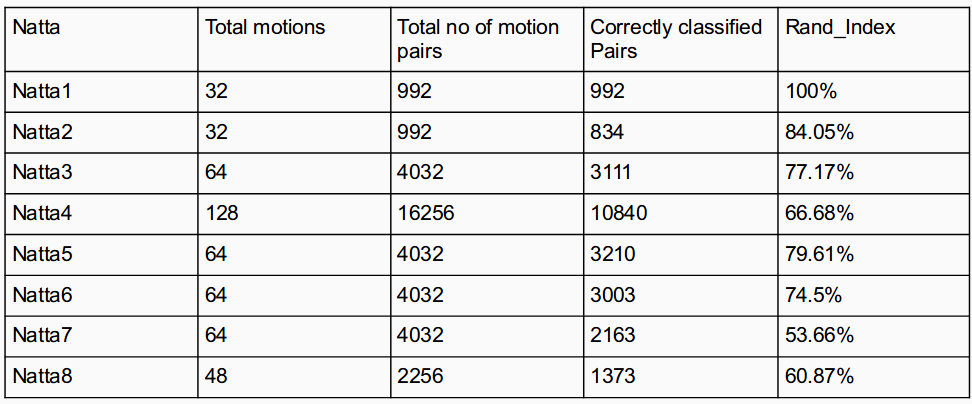
\includegraphics[width=140mm]{Pictures/res1.png}
\end{figure}


The accuracy is measured using the rand index as described in the previous chapter.We can observe the accuracy is really good for the simple motions in the initial Nattas.But as complexity of motions increases in the later nattas,the accuracy was decreased.We have analyzed reasons for less accuracy in the Analysis section.

\subsubsection{Similarity Matrix}
We can see the similarity matrix and observe the following point.Motion1 is similar with Motion5,Motion9,Motion13 which is evident by light colour in the figure.Motion0 is similar with Motion8.But because Motion4 is similar with Motion8,the Motion0,Motion4,Motion8 went into same cluster as we wanted.
\begin{figure} [H]
\centering
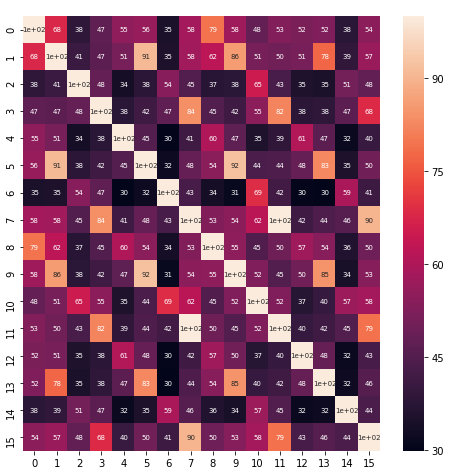
\includegraphics[width=90mm]{Pictures/sim.png}
\end{figure}
\subsubsection{Confusion Matrix}

\begin{figure} [H]
\centering
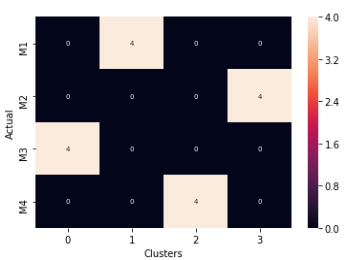
\includegraphics[width=85mm]{Pictures/confuse.png}
\end{figure}
Here you can see there are four motions of type M1 and every motion went into cluster 1.The results for other nattas and dancer can be found \href{https://docs.google.com/document/d/1tpQId7VadBUHFW8xKCehUH4VTjIplCjThj6Vl_HT_N4/edit}{here}.


\subsection{Different Variations tried}

Generally Histogram of Optical Flow is used in place of using dense optical flow directly.Hence, we tried to use HOF in place of Dense Optical Glow in the first step.Here,we tried two variations of HOF weighted binning and Interval binning.

\begin{figure} [H]
\centering
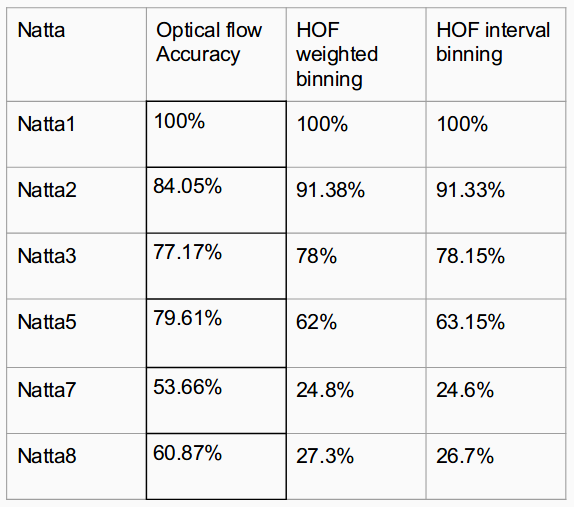
\includegraphics[width=80mm]{Pictures/res2.png}
\end{figure}

We have also tried varying binsizes to see how it affects accuracy. Increasing bin size decreases the accuracy of simple motions but increases the accuracy of complex motions.

\begin{figure} [H]
\centering
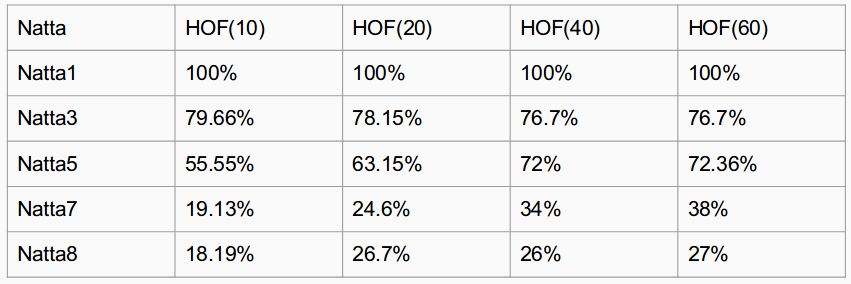
\includegraphics[width=120mm]{Pictures/res3.png}
\end{figure}

\subsection{Reasons for Low Accuracy for Natta7}

In Natta7, the number of frames for each motion differs too much.For example M1 contains 62 frames whereas M2 contains 4 frames 
Consider three motions M1,M2 and M1 in the next cycle
Since M2 has less frames DTW is assigning less cost to M1 and M2 rather than to M1 and M1 in the next cycle.So the motions with less no of frames are affecting the similarity matrix.

\textbf{Noisy Motions : } The motions having less than 10 frames are causing the accuracy to be low as explained above.Also it is highly impractical for a motion to be in such less no of frames. Hence we treat motions with less frames and removed them and recalculated accuracy for the above methods.

\subsection{Results without noisy motions}

\begin{figure} [H]
\centering
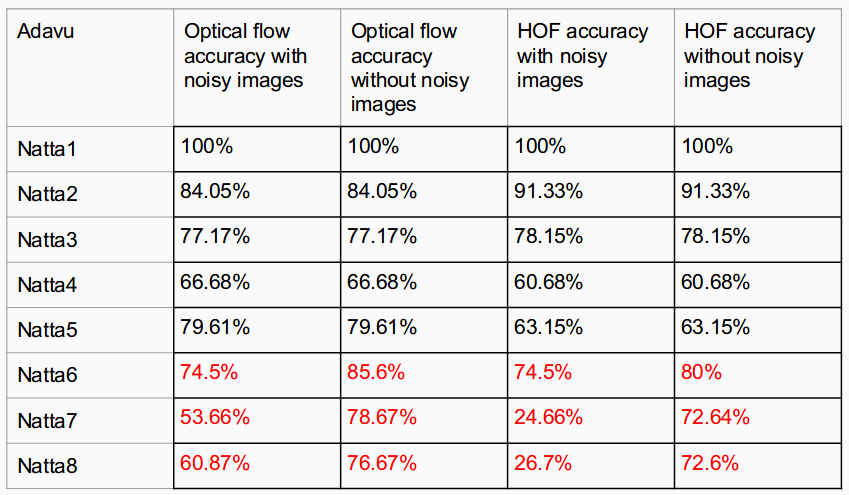
\includegraphics[width=120mm]{Pictures/res4.png}
\end{figure}


\section{Supervised Learning}

As we have seen dense optical flow as the better feature compared to HOF. we used dense optical flow for the feature extraction.But the problem is feature vector are of different sizes for different motions,we made all of them equal size by appending with a small value (1e-5).we then used SVM for classification.We have trained the svm on one performance of the dancer and tested on the other performance.

\subsection{SVM Results}

\begin{figure} [H]
\centering
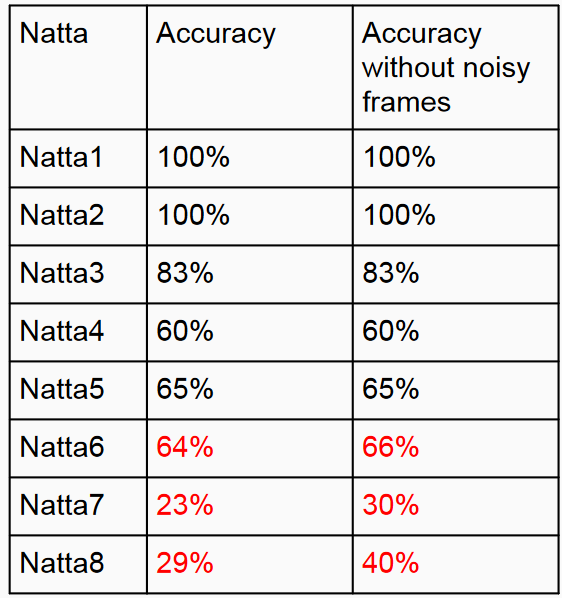
\includegraphics[width=80mm]{Pictures/res5.png}
\end{figure}

Here note that removing noisy motions doesn't increased accuracy much because noisy motions affect only the DTW Result.

\subsection{Approach 2 : K - Nearest Neighbour}

In this approach we have taken one performance of a dancer as training data and tested it on the other performance.For each motion in test data we assign it to the most similar motion in training set.The "most similar" is measured by Dense Optical Flow and DTW.

Here the removal of noisy frames had increased accuracy since here we used DTW and the noisy motions are effecting DTW result.

\begin{figure} [H]
\centering
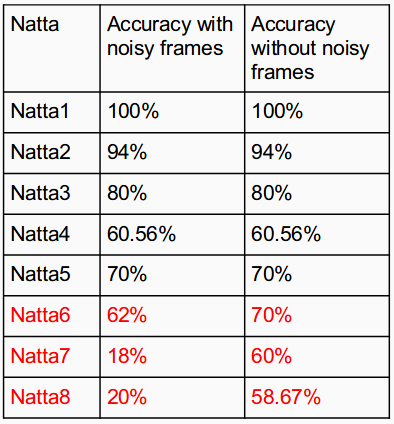
\includegraphics[width=80mm]{Pictures/KNN_res.png}
\end{figure}




\section{Conclusion \& Future Work }

In this work we tried  various approaches for clustering of motions.In the unsupervised approach, using dense optical flow we achieved an average accuracy of 81\% and by using HOF we achieved 77\% average accuracy.However using HOF decreased the running time of the algorithm by half since it decreases the feature vector size.we have also tried using SVM for classification but the accuracy was not so good.

In future,we want to automate the process to find optimal no of clusters in the video.we also wanted to extend this approach to skeletal videos.we aim to improve the SVM classification approach by training on more data.






